\documentclass[12pt]{amsart}
\pagestyle{empty}
\usepackage[margin = 1in]{geometry}
\usepackage{array}
\usepackage{amsmath}
\usepackage{caption}
\usepackage{subcaption}
\usepackage{graphicx}


\newcolumntype{M}{>{$}c<{$}}
\setlength{\parindent}{0mm}
\newcommand{\tab}{\hspace*{2em}}
\renewcommand*{\arraystretch}{1.5}
\newcommand{\comment}[1]{}

\title{A Stochastic Spatial Model for Tumor Growth}
\author{Aashiq Dheeraj, Rick Durrett}

\begin{document}
\maketitle


\section{Abstract}
Evolutionary game theory can be used to study the interactions of different cell phenotypes and describe tumor population dynamics. Instead of killing tumor cells, clinical treatment could aim to change the nature of the evolutionary game-- enabling healthy cells to select out malignant cells. Most applications of  evolutionary game theory to tumor growth have considered the tumor as a homogeneously mixing population that is governed by the replicator equation. We model the tumor population as an interacting particle system, with discrete individuals, stochastic local interactions, and explicit spatial consideration. Using this model, we see how predictions are changed when space is taken into account. In particular, we consider the analysis of multiple myelomas proposed by Dingli \cite{Dingli2009}, Basanta's work on glioma progression \cite{Basanta2008}, and the robust Hawk-Dove-Retaliator game \cite{Smith1986} . Our model agrees with Basanta's in that we should have coexistence between the three tumor phenotypes. Dingli's tumor population and the HDR game exhibit bistability in a certain parameter regime. Our spatial model predicts a transition between the two stable states at a critical parameter value, so there is no bistability. 

\section{Introduction}
	The theory of evolutionary games was introduced to study ecological competitions \cite{Smith1986}. However 15 years ago, Tomlinson suggested that it could be used to study interactions between tumour cells \cite{Tomlinson1997,TomBod}. More recently, Axelrod, Axelrod, and Pienta  \cite{Axelrod2006} have explained how the cooperation of cancer and normal cells can bring on mutually beneficial events such as angiogenesis (the development of blood vessels), Dingli et al (2009) have studied the interactions between osteoclast, osteoblasts, and tumor cells in multiple myeloma, and in a series of papers Basanta and coauthors have studied the role of glycolysis in glioma progression and invasion \cite{Basanta2008,Basanta2011}. All of these analyses assume that the population of cells is homogeneously mixing while in reality, each cells compete only with those nearby. Here we will investigate how predictions change when the space is take into account.
	
\section{Materials and Methods}
\subsection{Game Theoretic Model}
	First, consider a traditional EGT approach to the modeling. Suppose that we have $n$ cell types. Let $x_i$ denote the fraction of the population that is cell type $i$. We must have $\sum_{i=1}^n x_i = 1$.Then, the state of the population, $\vec{x}$ can be represented as a point on the $n$-dimensional simplex. 
	
	The time-evolution of this state is given by the replicator equation. For each $i$, $$\dot{x_i} = x_i (W_i(\vec{x}) - \overline{W})$$, where $W_i$ is the fitness of cell type $i$ and $\overline{W}$ is the average fitness. Suppose that the fitness payoff due to the interaction between cell types depends linearly on the cell proportions. We can write a payoff matrix, U, that captures the results of this interaction. Then $W_i(\vec{x}) = \vec{\textbf{e}}_i \cdot U\vec{x} $ and $\overline{W} = \vec{x}^\top U \vec{x}$.
	
\subsection{Spatial Refinement}



According to this model, the fitness of a given individual depends upon the state of the population as a whole. However, this fitness should only depend upon interactions with nearby neighbors. If the population is homogeneously mixing, the composition of the neighbors will look like the state, $ \vec{x} $. The replicator equation can then be viewed as a mean-field approximation to a spatial game. As shown by Durrett and Levine, including spatial effects can have important implications for the dynamics \cite{Durrett1994}.

We introduce a spatial stochastic model to study differences in the spatial case. In our model, cells are represented as points on the lattice $\mathbb{Z}^d$, initialized to one phenotype. The "neighborhood" of a given cell refers to the von Neumann neighborhood, consisting of the 2-4 cells with which it shares an edge. The "fitness" of a given cell is computed by summing over the payoffs for interactions with each neighbor. The payoffs are taken from the payoff matrix for the particular game under consideration. The time-evolution of the lattice is given by choosing a cell at random and replacing it with one of its neighbors, chosen at random. Each neighbor has probability of being chosen proportional to its fitness. 

\begin{figure}
\centering
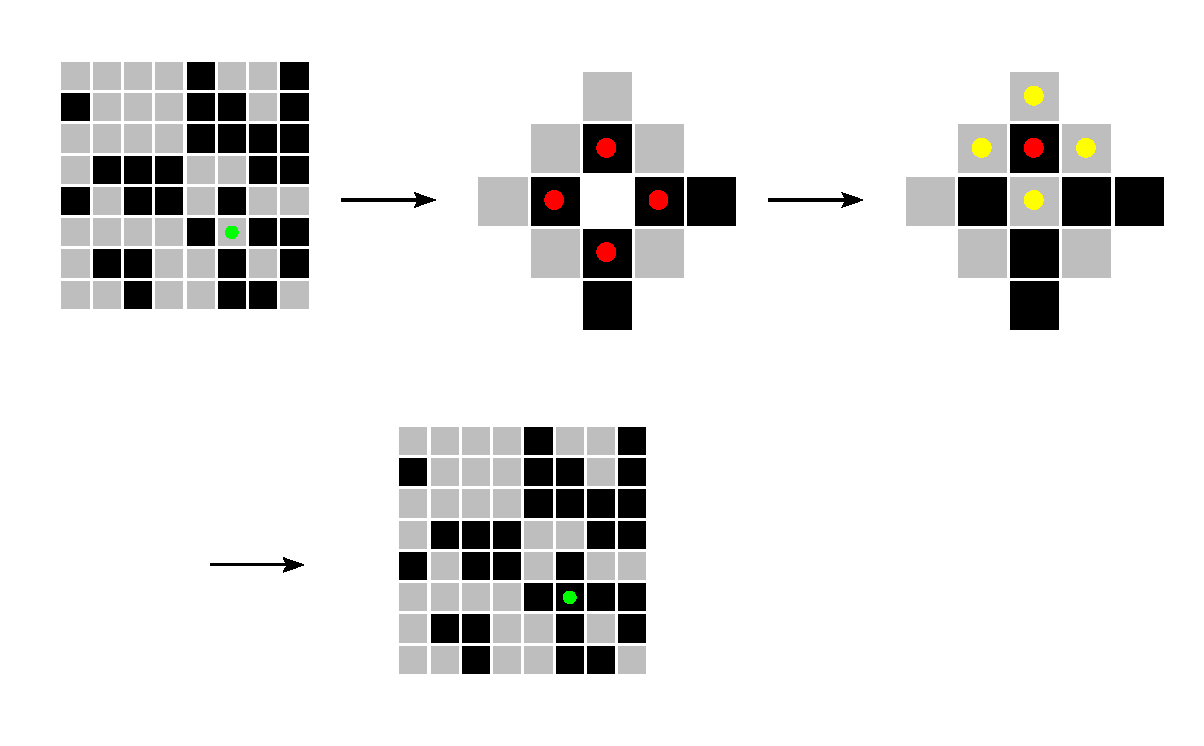
\includegraphics[width = \linewidth]{Diagrams/General/themodel}
\caption{An example of a Moran update. The cell marked green is randomly selected to die. The fitness of each red neighbor is computed using its yellow neighbors (including the dead cell). Finally, the update is made.}
\end{figure}

There are a few metrics one can use to characterize the behavior of our model. A good way to show coexistence is to look at cell type frequencies over time. If they are stable over long periods of time or have sustained oscillations, this might indicate coexistence. The lattice used must be large enough that stochastic fluctuations in population do not accidentally eliminate a cell type, in which case the predicted dynamics could be far off. As long as this is satisfied, the initial conditions should not matter. This is true of stochastic models as discussed in Durrett and Levin \cite{Durrett1994}, which have infinite size. The dynamics of interest tend to take place at a characteristic length scale, so the lattice we use must be large enough to capture them. To determine this, we need a metric to quantify the size of the structures we observe in the spatial model. We define the degree of clustering as the ratio of identical neighbor pairs to total neighbor pairs. If the clustering tends to keep increasing, this might indicate that the chosen lattice is  not large enough.

\subsection{Analytic Results}
We can use results from Cox, Durrett, and Perkins for voter model perturbations to look at spatial evolutionary games like the proposed model \cite{Cox2011}. 

\begin{figure}[t]
\caption{An example of a possible initial condition. Red, Green, and Blue represent different cell types. In spatial games, the arrangement and proportion of different cell types is generally unimportant in determining the outcome.}
\centering
\includegraphics[width = 2in]{Diagrams/General/even_random_mix}
\end{figure}

\section{Results}


\subsection{Case 1: Glioma Progression}
Basanta \textit{et al.} used EGT to study interactions between different tumor cell phenotypes found in glioblastomas. They were able to explain several observed features of glioma progression, such as a switch to glycolytic respiration. In their model, there are three tumor phenotypes: autonomous growth (AG), invasive (INV), and glycolytic metabolism (GLY). Glycolytic metabolism is less efficient than aerobic respiration, and cells generally adopt it when a tumor is insufficiently oxygenated. Let $k$ represent the fitness cost of switching to glycolytic respiration. GLY cells tend to acidify the pH of the surrounding microenvironment, granting a payoff $n$ to themselves, as well as a cost $n$ to non-GLY cells. Finally, INV cells are expected to flee upon encountering another type. They should obtain the base payoff minus the cost of motility, $c$. Thus, we have the following payoff table. 

$$A = \bordermatrix{\text{}& AG & INV & GLY\cr
                AG & \frac{1}{2} & 1 & \frac{1}{2} - n \cr
                INV & 1 - c  &  1 - \frac{c}{2} & 1 - c \cr
                GLY & \frac{1}{2}+n-k & 1-k & \frac{1}{2}-k \cr
               }$$


% \begin{table}[h]
% \caption{Payoff Matrix}
% \centering

% \begin{tabular} {c | MMM}


% & AG & INV & GLY\\
% \hline
% AG& \frac{1}{2} & 1 & \frac{1}{2} - n\\
% INV & 1-c & 1-\frac{c}{2} & 1-c\\
% GLY & \frac{1}{2}+n-k & 1-k & \frac{1}{2}-k\\

% \end{tabular}
% \label{tab:hresutl}
% \end{table}

Adding appropriate constants to the columns, we have the payoff 

In his 2008 paper, Basanta considers the replicator dynamics for this system, without considering spatial effects. He computes the location of an internal fixed point and gives constraints for its existence. As shown by Hofbauer and Sigmund, if there is an evolutionarily stable internal fixed point, then it is globally stable. However, Basanta does not address the stability of his point. In the case that the fixed point is not evolutionarily stable, it \cite{Hofbauer1998} has little value in predicting the behavior of either the uniformly mixing case considered by Basanta or the spatial case. 

In order to characterize the fixed point, we compute it from the replicator equation, linearize around it, and consider the eigenvalues of the Jacobian.
Let $\vec{p} = { \begin{pmatrix} p_1 & p_2 & 1-p_1-p_2 \end{pmatrix}}^\top$, noting that the frequencies of all the cell types must add to 1. Then, $$\vec{W} = A\vec{p} = 
{\begin{pmatrix} \frac{p_2}{2} + p_1 n + \frac{1}{2}-n\\
1-c + \frac{p_2 c}{2}\\ %compute W, Wbar
p_1*n+\frac{p_2}{2} + \frac{1}{2}-k \end{pmatrix}}$$. The average fitness is given by  $$\overline{W} = \vec{p}^\top A \vec{p} = \frac{1}{2}-k+ k p_1 + p_2 (1 - c + k) - \frac{p_2^2}{2} (1-c) $$

To solve for the fixed point, we set $W_1 = \overline{W}$ and $W_2 = \overline{W}$, yielding the internal fixed point 
$$p^* = {\begin{pmatrix}\displaystyle{\frac{2 n k + k - n c - k c}{2n^2}}\\
		\displaystyle{\frac{n-k}{n}}\\
		\displaystyle{\frac{k c - k + c n}{2n^2}}
		\end{pmatrix}}$$
Since each component of $p^*$ must fall in the range (0,1), we must have one of the following sets of constraints on $c$,$n$, and $k$: \\
\{$\displaystyle{0 < c \ge \frac{1}{2}}$, $\displaystyle{\frac{c n}{2 n - c + 1} < k < \frac{c n}{1-c}}$\} \tab OR \\
\{$\displaystyle{\frac{1}{2} < c < \frac{1 + 2n}{2}}$, 
$\displaystyle{\frac{c n}{1 + 2n - c} < k < n}$\}

We can linearize around this fixed point in order to compute its stability. The Jacobian must have negative real part when evaluated at $p^*$. Solving, $p^*$ is only unstable for $c > 1$, $n > c - \frac{1}{2}$. The term $c$ represents the cost of motility, so it is not biologically realistic for it to be larger than 1, the base payoff. Thus, as long as the fixed point $p^*$ exists, it is stable.

Stable fixed points of the replicator equation on the inside of the simplex are unique and globally asymptotically stable \cite{Hofbauer1998}. The existence of such a point in the mean-field ODE suggests coexistence in the stochastic spatial model \cite{Durrett2009}. Thus, we expect AG, INV, and GLY to coexist for some parameter regime in our model.


\begin{figure}[ht]

	\begin{subfigure}[b]{0.4 \textwidth}
		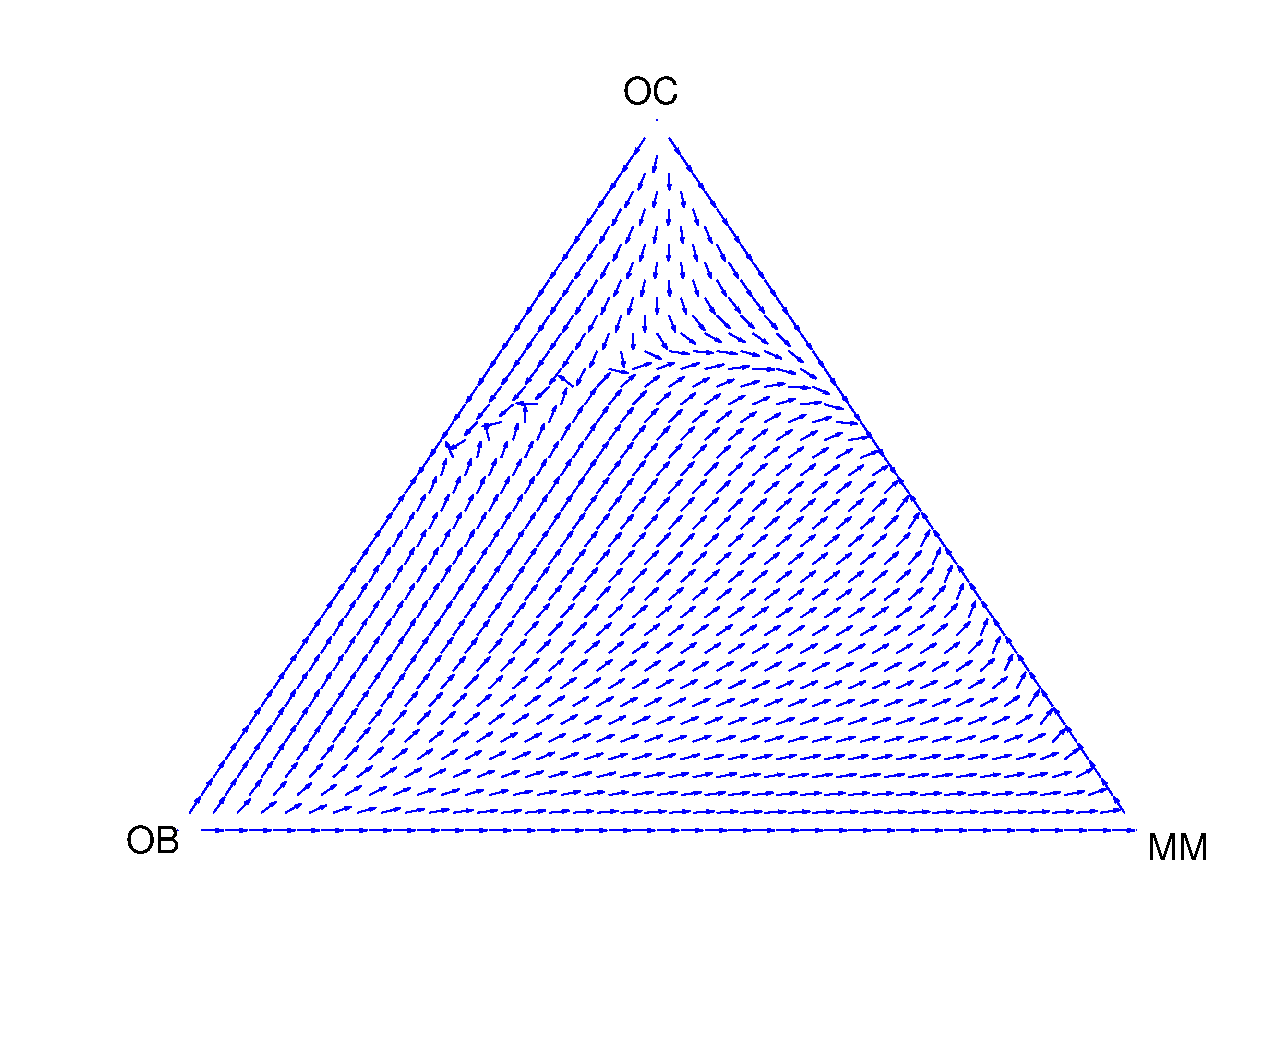
\includegraphics[width = 0.9 \textwidth]{Diagrams/Basanta/phase}
		\caption{Phase Portrait has attracting fixed point, implying coexistence}
	\end{subfigure}
	~
	\begin{subfigure}[b]{0.4 \textwidth}
		\includegraphics[width = 0.9 \textwidth]{Diagrams/Basanta/sample}
		\caption{Sample Output. Cells of type AG are red, INV green and GLY blue.}
	\end{subfigure}

	\begin{subfigure}[b]{0.4 \linewidth}
		\includegraphics[width = 0.9 \linewidth]{Diagrams/Basanta/"Basanta-c-0_3-n-0_5-k-0_2_freqs"}
		\caption{Unexpectedly, INV cells dominate}
	\end{subfigure}
	~
	\begin{subfigure}[b]{0.4 \linewidth}
		\includegraphics[width = 0.9 \linewidth]{Diagrams/Basanta/Basanta1_clustering}
		\caption{Clustering over time}
	\end{subfigure}

\caption{if this works...}
\end{figure}

  	


\subsection{Case 2: Multiple Myeloma}
In a 2009 paper, Dingli applies EGT to multiple myeloma evolution \cite{Dingli2009}. Multiple myeloma (MM) cells interact with the body's osteoclast (OC) and osteoblast(OB)cells, which are important in normal bone remodelling. When there are no MM cells, there is a stable equilibrium between OC and OB cells. MM cells promote the growth of OC cells by secreting osteoclast activating factors (OAF's) like interleukin  1$\beta$, RANKL, and MIP-1$\alpha$. MM cells also hinder OB differentiation by secreting Dickkopf-1 \cite{Dingli2009}. OC cells produce IL-6 and osteopontin to promote MM growth. The frequency-dependent interactions of the three cell types can be treated as an evolutionary game with a payoff matrix encapsulating the above information. Dingli further assumes that interactions between cells of the same type incur no cost or benefit. We can write the following payoff matrix, which captures the result of these interactions. 

$$A = \bordermatrix{\text{}&OC&OB&MM\cr
                OC& 0 & a& b \cr
                OB& e  &  0 & -d \cr
                MM& c & 0 & 0 \cr
               }$$

Dingli reduces the above matrix, $A$, to the minimal matrix, $B$, through the projective transformation $B_{ij} = \frac{A_{ij}}{\phi_j}$ where 
$\phi = {\begin{pmatrix} e & a & \frac{be}{c} \end{pmatrix}}$.
This yields the minimal matrix
$B = {\begin{pmatrix}
0 & 1 & \beta \\
1 & 0 & -\delta \\
\beta & 0 & 0
\end{pmatrix}}$. 
The projective transformation moves any internal fixed point into the barycenter of the simplex without changing the replicator dynamics or stability \cite{Hofbauer1998}. The dynamics can be divided into three regimes. For $\beta < 1 and \beta + \delta < 1$, an equilibrium between OC and OB is a globally attracting fixed point. For $\beta > 1$, an OC-MM equilibrium is globally attracting. Finally, for $\beta < 1 and \beta + \delta < 1$, we have bistability between an OB-OC equilibrium and an OC-MM equilibrium. 
\begin{figure}[htb]
\caption{Sample Phase Portrait for  $\beta < 1 and \beta + \delta < 1$  }
\centering
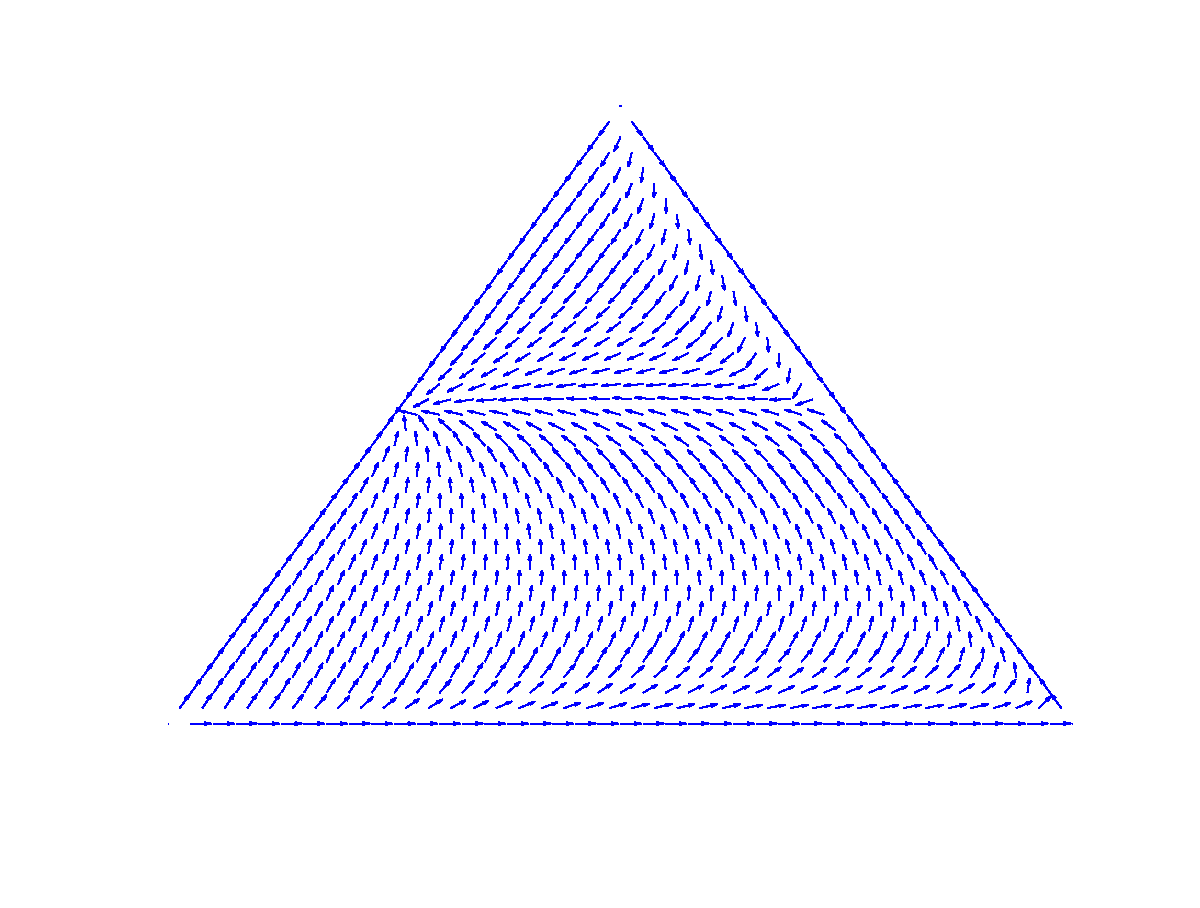
\includegraphics[width = 1.5 in]{Diagrams/Dingli/OCOB}
\end{figure}

\begin{figure}[htb]
\caption{Sample Phase Portrait for  $\beta < 1 and \beta + \delta > 1$  }
\centering
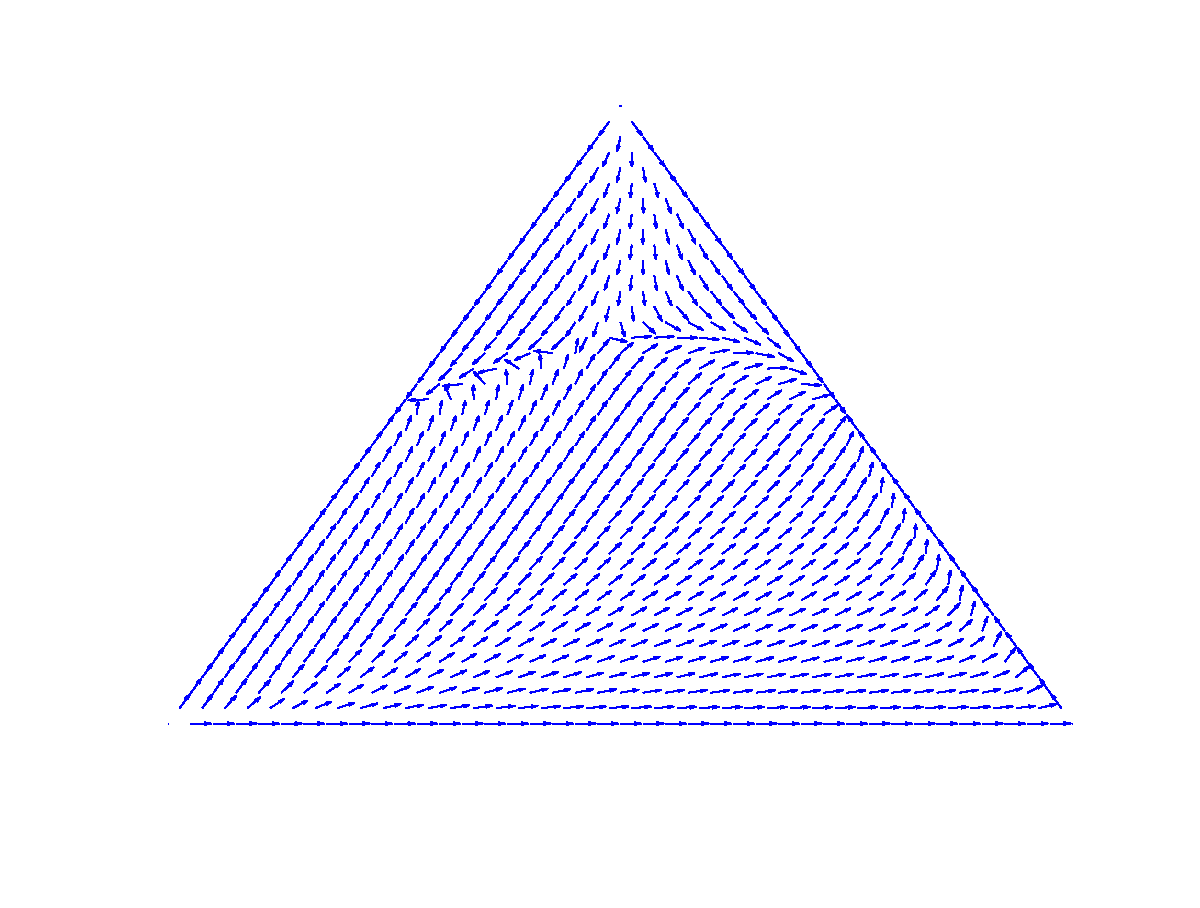
\includegraphics[width = 1.5 in]{Diagrams/Dingli/bistable}
\end{figure}

\begin{figure}[htb]
\caption{Sample Phase Portrait for  $\beta > 1$}
\centering
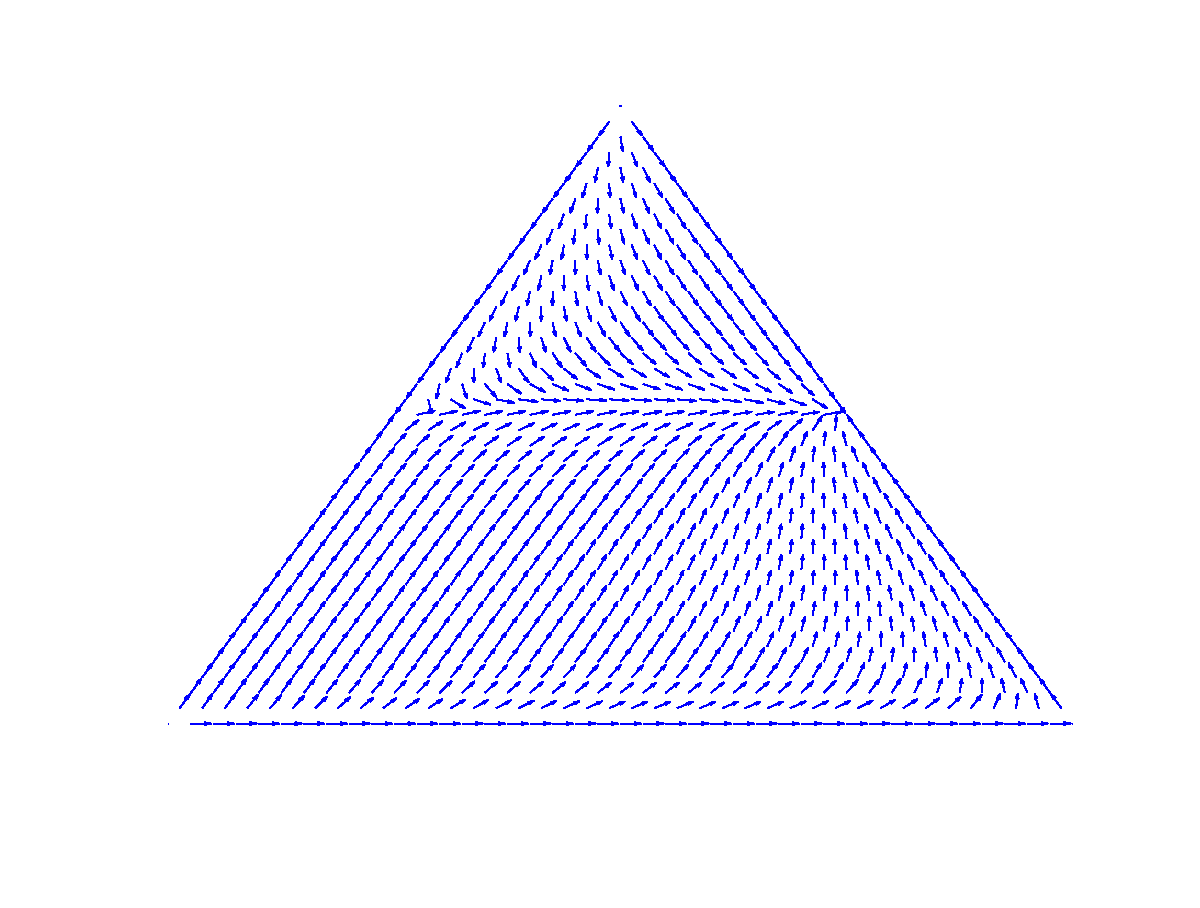
\includegraphics[width = 1.5 in]{Diagrams/Dingli/OCMM}
\end{figure}

In the spatial treatment, phase portraits with a globally attracting equilibrium should result in coexistence between the relevant types \cite{Durrett2009}. Indeed, phase portraits with OB-OC or OC-MM equilibria result in the same outcome for the spatial case. For $\beta < 1$ and $\beta + \delta > 1$, the replicator equation suggests that the location of the initial condition with respect to the saddle point should determine which basin of attraction the system falls into. 
Our model shows that for each $\beta$, there is a critical $\delta$ at which the system switches from an OC-OB equilibrium to an OC-MM equilibrium. In addition, there is a critical $\beta$ below which we will always have an OC-OB equilibrium for any choice of $\delta$.
\comment{
\begin{figure}[htb]
\caption{Sample output for $\beta < 1$ and $\beta + \delta > 1$}
\centering
\includegraphics[width = 1.5 in]{Diagrams/Dingli/sample}
\end{figure}

\begin{figure}[htb]
\caption{For each $\beta$, there is a critical $\delta$ below which OB always wins. There is also a critical $\beta$ (0.35) below which there is no $\delta$ for which MM wins.}
\centering
\includegraphics[width = 1.5 in]{Diagrams/Dingli/critdeltavsbeta}
\end{figure}
}


\pagebreak

\subsection{The Effect of Space on Cell Frequencies}
The model suggests that spatial considerations increase the importance of cooperativity between cell types. Phenotypes that exhibit cooperativity make up a higher proportion of the population than the mean-field case might predict. For example, consider the game given by the payoff matrix
$$A = {\begin{pmatrix}
  0 & 1\\
  0 & 1 \\
\end{pmatrix}}$$

In this case, there are two phenotypes. Call them ant and spider. Spiders receive a fitness payoff from pairwise interactions with ants, so their fitness is highest when surrounded by ants. Ants receive a payoff from interactions with other ants, as one might find in an anthill. Thus, in the spatial case, ants should tend to cluster together. In the mean-field approximation, this clustering cannot occur, as the population is assumed to be homogeneously mixing. Furthermore, the dynamics are invariant under addition of a constant to a column. Thus, the matrix A is equivalent to the zero matrix in the mean-field approximation. This represents completely random selection. In the spatial case, such a system should behave like the voter model-- with constant cell proportions and increasing clustering.



\section{Conclusion}
We have created a stochastic spatial model for a generic evolutionary game and applied it to the interplay of phenotypes in tumor growth. Our model shows that explicit spatial considerations can change the qualitative behavior of an evolutionary game. If the mean-field phase portrait has a globally stable fixed point, the spatial model has coexistence between the represented cell types. On the other hand, if there is bistability, spatial considerations show a transition between stable fixed points. 

\pagebreak


\newpage \bibliographystyle{plain}
\bibliography{bibliog}

\end{document}






		